\chapter[Materiais e Métodos]{Materiais e Métodos}
\label{materiais-e-metodos}

Este capítulo descreve o conjunto de dados elaborado, a arquitetura da rede neural e o método de segmentação proposto.

\section{Conjunto de dados}

As imagens utilizadas foram obtidas a partir do fêmur esquerdo de um rato \textit{Rattus norvegicus} da linhagem \textit{Wistar} saudável com 200 - 250g. O animal foi sacrificado e os fêmures foram removidos e fixados em formaldeído 10\%, tamponado e desmineralizado em EDTA 4,13\%. A diáfise (Figura~\ref{fig:estrutura-ossos-longos}), região intermediária do fêmur, foi incluída em parafina e obteve-se cortes histológicos seriados de cerca de 5 micrômetros de espessura corados em \ac{HE}, que é o tipo de coragem mais amplamente utilizado na histologia devido à sua simplicidade e ao grande número de estruturas do tecido que permite visualizar \cite{feldman2014tissue}. 

Todos os procedimentos para se obter este material foram executados de acordo com as normas do Colégio Brasileiro de Experimentação Animal (COBEA), com aprovação do Comitê de Ética no Uso de Animais da Universidade Federal de Uberlândia (CEUA-UFU) -- Protocolo 060/09.

Neste estudo foram analisados 65 cortes histológicos de fêmur esquerdo. Foi utilizado um ScanScope AT Turbo\textregistered Scanner (Leica Biosystems, Nussloch, Alemanha) para digitalizar as imagens com uma ampliação efetiva de 20×. As imagens foram exportadas em arquivos TIFF de alta resolução. A Figura \ref{fig:original-images} mostra um exemplo de corte histológico para o fêmur irradiado. O tamanho da imagem na Figura \ref{fig:original-images}(a) é de 7.940 × 9.051 pixels, a largura e altura do pixel são 0,502 \(\mu\)m. Nessa resolução é possível identificar os canais ósseos (Figura \ref{fig:original-images}(b)).

\begin{figure}[h]
    \center
    \begin{tabular}{@{}c@{}}
        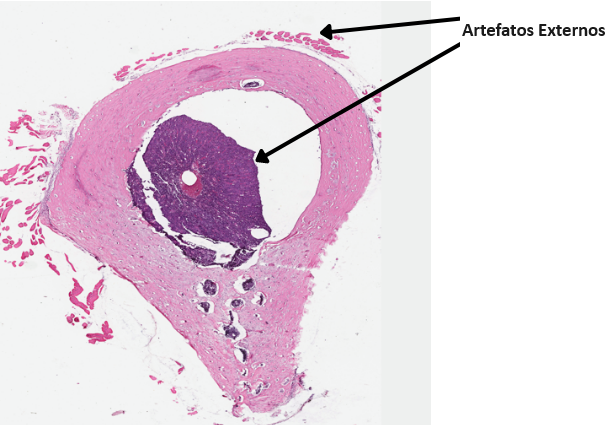
\includegraphics[width=0.45\textwidth]{figures/3_methods/imagem_original_inteira.png}
        \\[\abovecaptionskip]
    \small (a) Imagem original lâmina inteira
    \end{tabular}
    \begin{tabular}{@{}c@{}}
        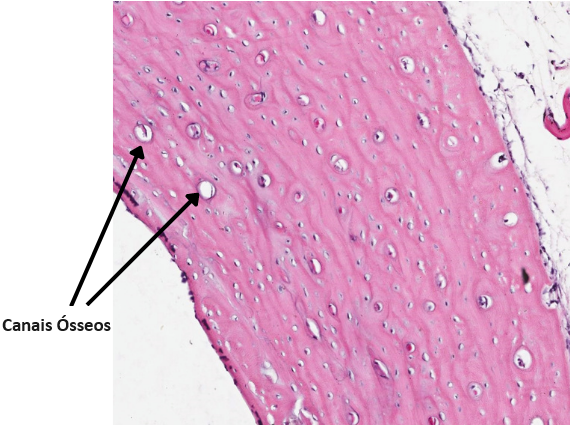
\includegraphics[width=0.45\textwidth]{figures/3_methods/imagem_original_ampliada.png}
        \\[\abovecaptionskip]
    \small (b) Imagem original ampliada
    \end{tabular}
    
    \caption[Exemplo de imagem utilizada no método proposto.]{Exemplo de imagem utilizada no método proposto. Em (a) imagem da secção inteira destacando artefatos externos que não são de interesse na análise, em (b) imagem ampliada destacando os canais ósseos.} 
    \label{fig:original-images}
\end{figure}

Todas as imagens coletadas foram marcadas por um especialista em histologia. A marcação foi feita por meio do software Photoshop\textregistered, versão 2016, contornando manualmente os canais ósseos com a ferramenta `Laço'. Em seguida foram exportadas em formato JPEG. Nesta etapa também foi feita a remoção do fundo da imagem, removendo artefatos externos que não eram interessantes para a análise. Os cortes histológicos marcados manualmente foram posteriormente divididos em 2037 sub-imagens de dimensões 640x640 pixels conforme será descrito adiante no texto.
A Figura \ref{fig:labelled-images}(a) apresenta um exemplo de imagem marcada, e a Figura \ref{fig:labelled-images}(b) uma região ampliada da mesma imagem evidenciando as marcações. 

As imagens de lâmina inteira bem como as sub-imagens utilizadas neste trabalho estão disponíveis publicamente no endereço: \href{https://www.kaggle.com/datasets/igorgonribsilva/histological-bone-canals-wsi}{https://www.kaggle.com/datasets/igorgonribsilva/histological-bone-canals-wsi}.

\begin{figure}[h]
    \center
    \begin{tabular}{@{}c@{}}
        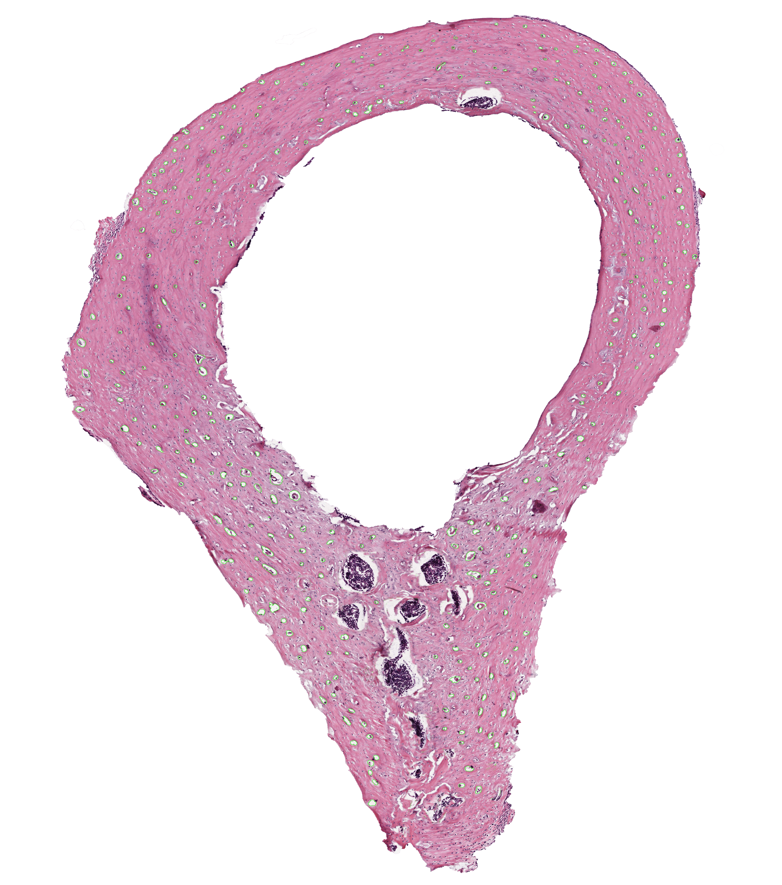
\includegraphics[width=0.45\textwidth]{figures/3_methods/imagem_marcada_inteira.png}
    \end{tabular}
    \begin{tabular}{@{}c@{}}
        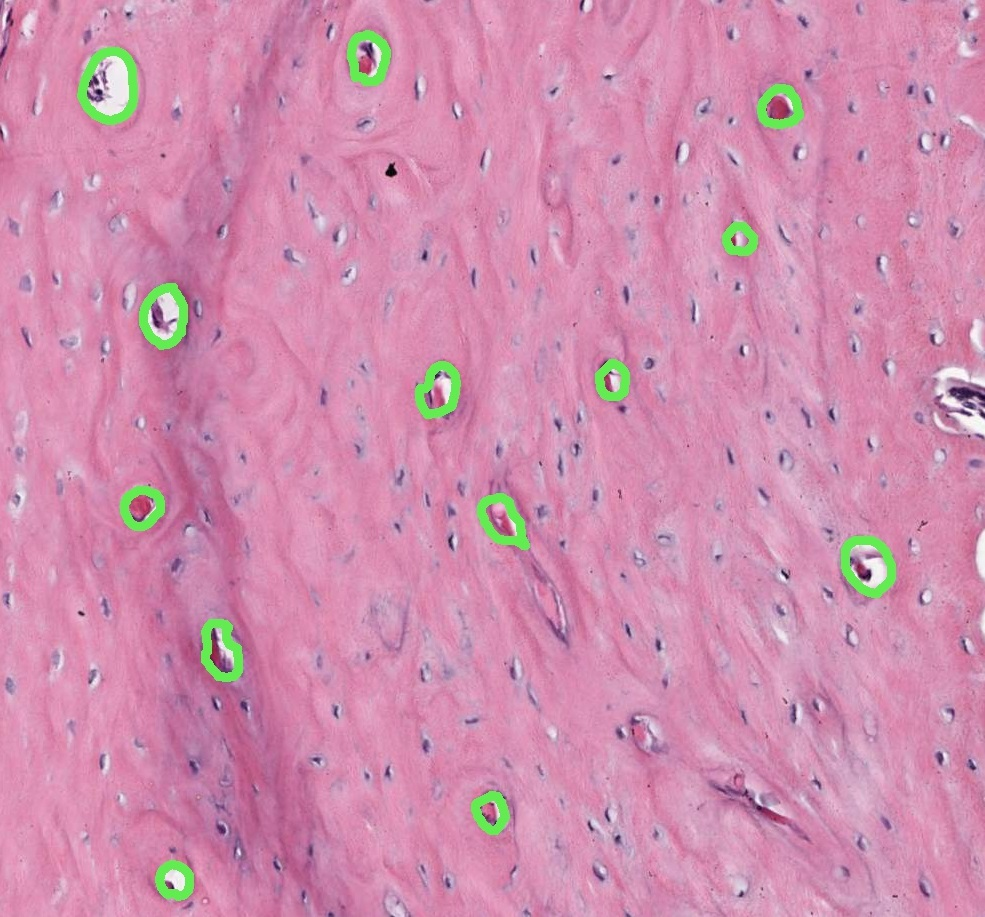
\includegraphics[width=0.45\textwidth]{figures/3_methods/imagem_marcada_ampliada.jpg}
    \end{tabular}
  
    \caption[Marcação do especialista para o método proposto.]{Imagem marcada por especialista. À esquerda a imagem inteira. À direita a imagem ampliada destacando os canais ósseos, contornados em verde.}
    \label{fig:labelled-images}
\end{figure}

\section{Arquitetura da Rede Neural}
A rede utilizada por este método foi a mesma desenvolvida por \cite{santos2022automated} com os mesmos parâmetros internos. Tal rede por sua vez é baseada na rede U-Net originalmente proposta por \cite{ronneberger2015u} com algumas modificações que estão destacadas na Figura \ref{fig:dali-unet} e serão descritas a seguir:

\begin{figure}[H]
  \centering
  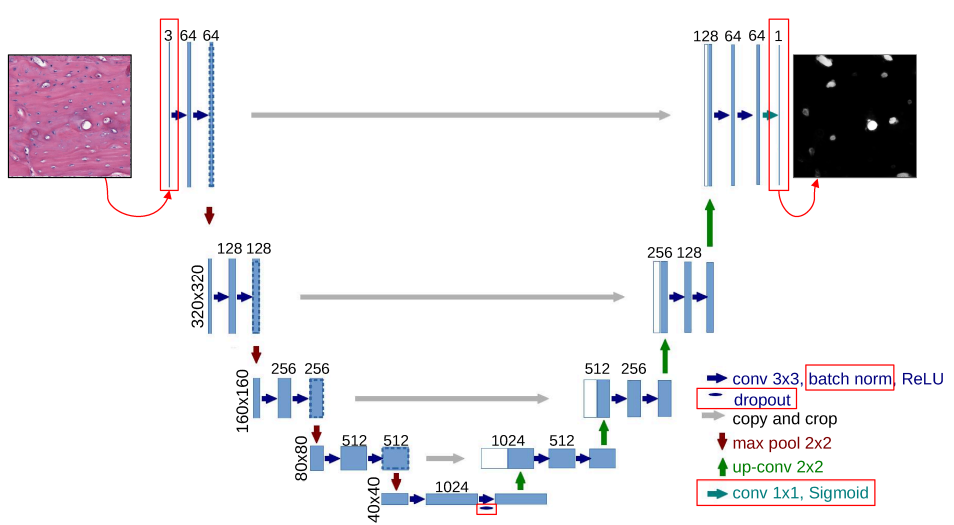
\includegraphics[width=.9\linewidth]{figures/3_methods/unet.png}
  \caption[Arquitetura da rede utilizada]{Arquitetura da rede utilizada baseada na rede U-Net original com modificações destacadas em vermelho. Imagem adaptada de \cite{santos2022automated}.}
  \label{fig:dali-unet}
\end{figure}

 \begin{itemize}
   \item Normalização em lote: A normalização em lote normaliza as entradas evitando valores muito baixos que possam gerar gradiente de fuga e fazer com que os pesos não se atualizem (ou se atualizem muito lentamente) durante o treinamento. A técnica também evita valores muito altos que possam gerar explosão de gradiente fazendo com que os pesos assumam valores muito altos rapidamente prejudicando o treinamento \cite{geron2019maos}. A normalização em lote foi aplicada após cada camada convolucional.
   \item \textit{Dropout}: O \textit{dropout} é uma técnica que consiste em desativar parte dos neurônios da camada conectada durante algumas etapas do treinamento a fim de evitar o sobreajuste, tornando a rede mais robusta e generalizável \cite{geron2019maos}. Foi utilizada uma taxa de \textit{dropout} de 0,5. Dessa forma a cada passo do treinamento metade dos neurônios eram desativados aleatoriamente para minimizar as chances de sobreajuste.
   \item Convolução 1x1 com função de ativação Sigmoid: Ao final do processamento, foi adicionada à última convolução (1x1) uma função de ativação Sigmoid a fim de que, ao invés de uma imagem binária, a saída da rede fosse uma imagem em escala de cinza onde quanto mais próxima de branco a cor de um pixel maior a probabilidade de o mesmo pertencer à região de interesse.
 \end{itemize}



\section{Método}
\label{method}
A fim de reaproveitar a rede neural proposta por \cite{santos2022automated}, foi necessário transformar as imagens marcadas manualmente em imagens binárias que destacassem as regiões de interesse. A Figura \ref{fig:preprocessing-steps} mostra uma marcação manual e a respectiva máscara binária gerada.

\begin{figure}[h]
    \center
    \begin{tabular}{@{}c@{}}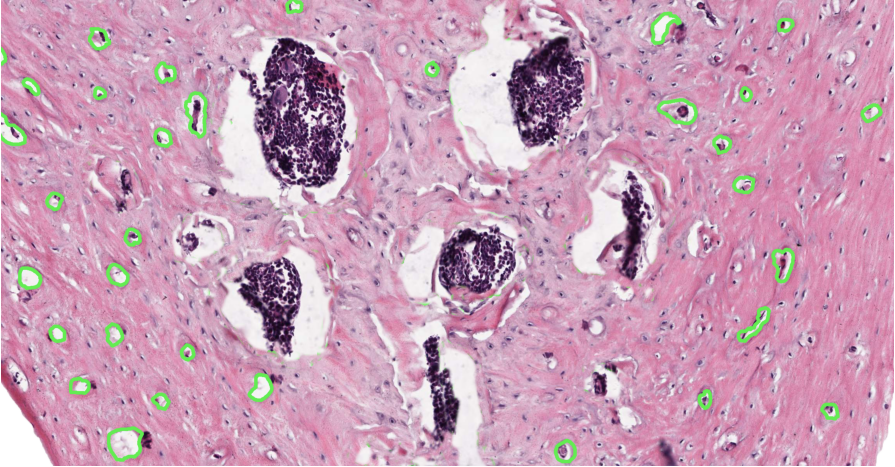
\includegraphics[width=0.45\textwidth]{figures/3_methods/preprocess/preprocess_step_0.png}
    \end{tabular}
    \begin{tabular}{@{}c@{}}
        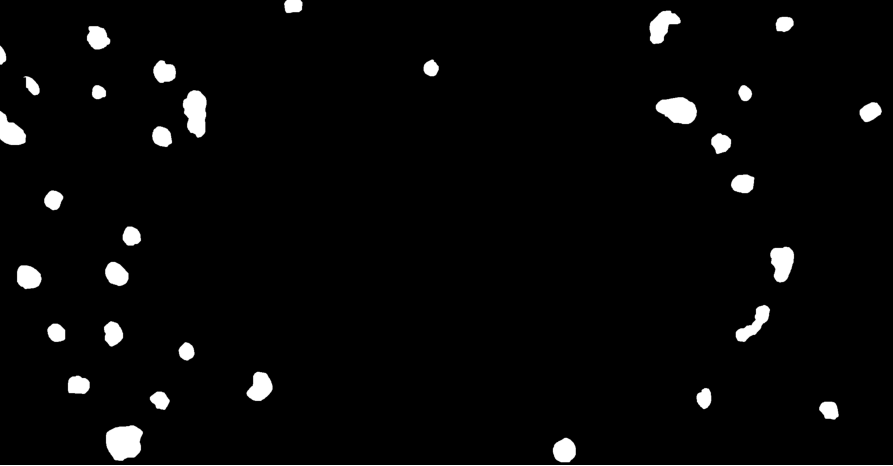
\includegraphics[width=0.45\textwidth]{figures/3_methods/preprocess/preprocess_step_3.png}
    \end{tabular}
  
    \caption[Região de imagem marcada manualmente e sua respectiva máscara binária.]{Região de imagem marcada manualmente (a) e sua respectiva máscara binária (b).}
    \label{fig:preprocessing-steps}
\end{figure}

O fundo das imagens originais (sem marcações) foi removido utilizando do processo descrito por \cite{santos2022automated}: diminuindo-se a escala das imagens por um fator de 32x, destacando-se a região com tecido por meio de um filtro de cor e mapeando-se a região selecionada na imagem em tamanho real.

Ainda como foi feito por \cite{santos2022automated}, são geradas sub-imagens a partir das imagens originais, desconsiderando-se as regiões que não contém tecido. O tamanho de sub-imagens utilizado foi 640x640 pixels, visto que foi o tamanho que apresentou melhores resultados em \cite{santos2022automated}. As sub-imagens que continham apenas fundo foram descartadas.

O treinamento ainda conta com a estratégia de aumento de dados utilizada por \cite{Santos2023a}, em que a cada época é aplicada uma transformação selecionada aleatoriamente. Para este aumento de dados, as seguintes operações foram consideradas: Inversão Horizontal, Inversão Vertical, Rotação, Tranposição, Transformação elástica, Distorção de grade e Distorção ótica. A Figura \ref{fig:aug-examples} mostra exemplos de cada uma dessas operações em comparação com um exemplar de sub-imagem original.

\begin{figure}[h]
    \center
    \begin{tabular}{@{}c@{}}
        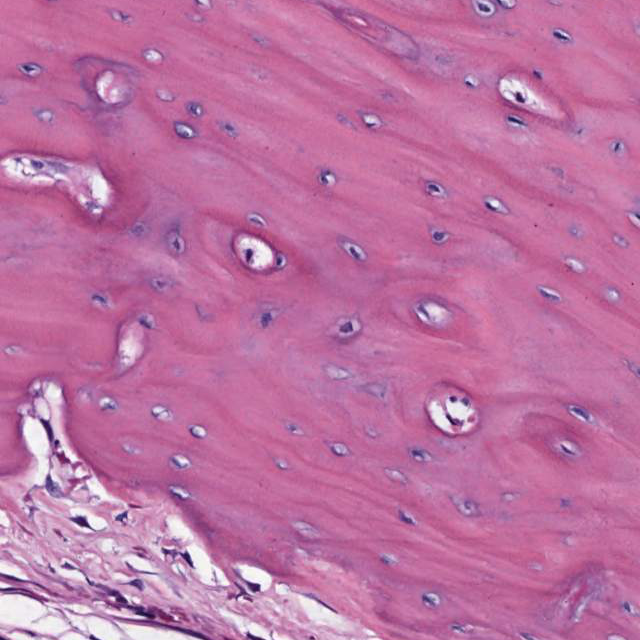
\includegraphics[width=0.2\textwidth]{figures/3_methods/transformations/205_r3c7.png}\\[\abovecaptionskip]
    \small (a) Imagem Original
    \end{tabular}
    \begin{tabular}{@{}c@{}}
        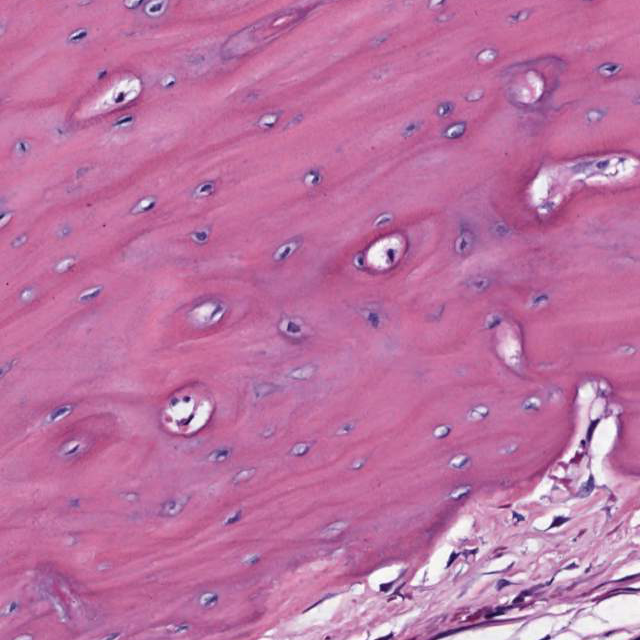
\includegraphics[width=0.2\textwidth]{figures/3_methods/transformations/205_r3c7_hflip.png}\\[\abovecaptionskip]
    \small (b) Inversão Horizontal
    \end{tabular}
    \begin{tabular}{@{}c@{}}
        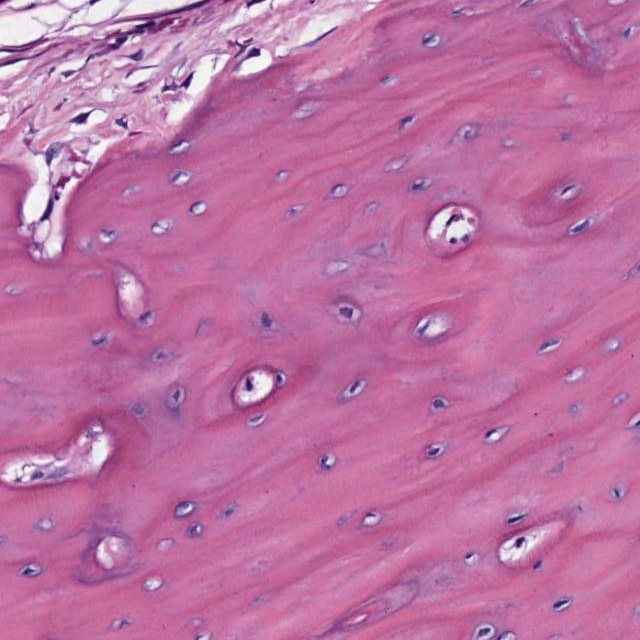
\includegraphics[width=0.2\textwidth]{figures/3_methods/transformations/205_r3c7_vflip.png}\\[\abovecaptionskip]
    \small (c) Inversão Vertical
    \end{tabular}
    \begin{tabular}{@{}c@{}}
        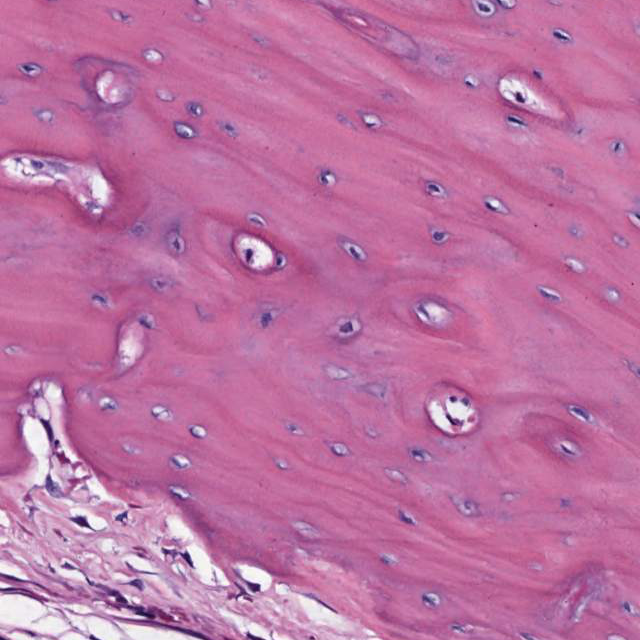
\includegraphics[width=0.2\textwidth]{figures/3_methods/transformations/205_r3c7_rotation.png}\\[\abovecaptionskip]
    \small (d) Rotação
    \end{tabular}

    
    \begin{tabular}{@{}c@{}}
        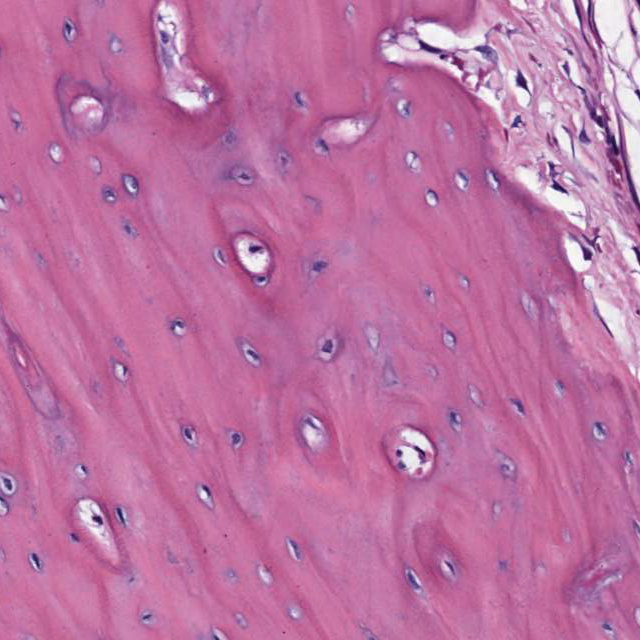
\includegraphics[width=0.2\textwidth]{figures/3_methods/transformations/205_r3c7_transpose.png}\\[\abovecaptionskip]
    \small (e) Tranposição
    \end{tabular}
    \begin{tabular}{@{}c@{}}
        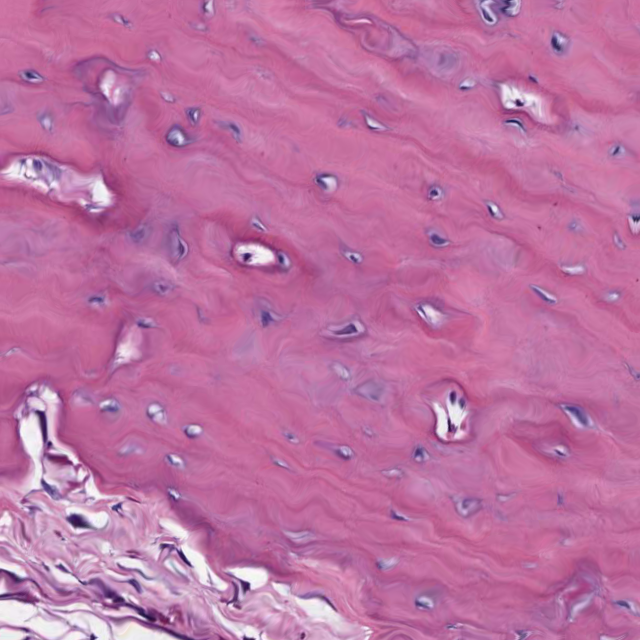
\includegraphics[width=0.2\textwidth]{figures/3_methods/transformations/205_r3c7_elastic_transformation.png}\\[\abovecaptionskip]
    \small (f) Transformação elástica
    \end{tabular}
    \begin{tabular}{@{}c@{}}
        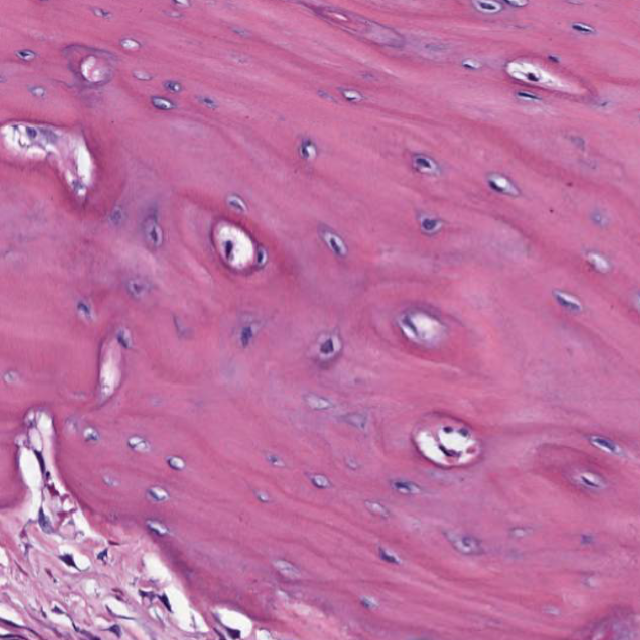
\includegraphics[width=0.2\textwidth]{figures/3_methods/transformations/205_r3c7_grid_distortion.png}\\[\abovecaptionskip]
    \small (g) Distorção de grade
    \end{tabular}
    \begin{tabular}{@{}c@{}}
        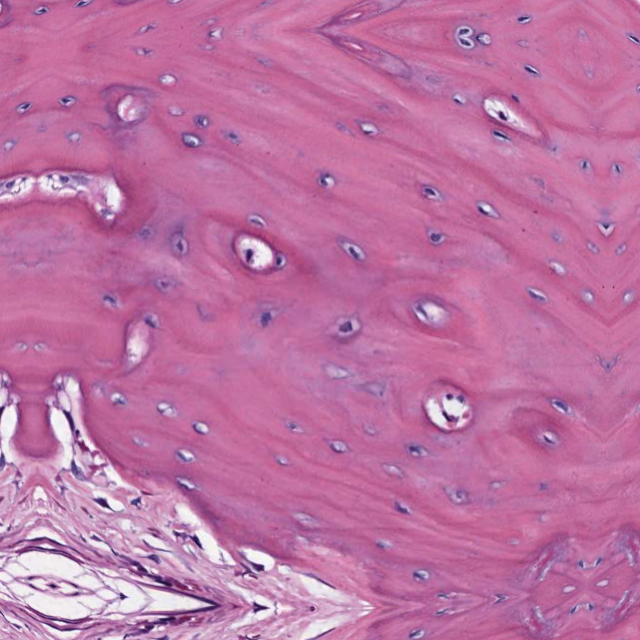
\includegraphics[width=0.2\textwidth]{figures/3_methods/transformations/205_r3c7_optical_distortion.png}\\[\abovecaptionskip]
    \small (h) Distorção ótica
    \end{tabular}
  
    \caption{Transformações utilizadas no aumento de dados.}
    \label{fig:aug-examples}
\end{figure}

 O conjunto de dados de treinamento foi composto por 80\% das sub-imagens, destas, 20\% foram usados para validação da rede durante o treinamento. Os 20\% restantes compuseram o conjunto de teste.

% Please add the following required packages to your document preamble:
% \usepackage[table,xcdraw]{xcolor}
% If you use beamer only pass "xcolor=table" option, i.e. \documentclass[xcolor=table]{beamer}
% \begin{table}[h]
% \center
% \begin{tabular}{|l|l|l|l|l|}
% \hline
% \rowcolor[HTML]{C0C0C0} 
% \textbf{Patch Size}                        & \textbf{WSI Images} & \textbf{Patches} & \textbf{Training Set}     & \textbf{Test Set} \\ \hline
% \cellcolor[HTML]{EFEFEF}\textbf{140x140}   & 100                 &                  &                           &                   \\ \cline{1-5}
% \cellcolor[HTML]{EFEFEF}\textbf{320x320}   & 100                 &                  &                           &                   \\ \cline{1-5}
% \cellcolor[HTML]{EFEFEF}\textbf{640x640}   & 100                 & 1722             & 1258 (315 for validation) & 464               \\ \cline{1-5}
% \cellcolor[HTML]{EFEFEF}\textbf{1200x1200} & 100                 &                  &                           &                   \\ \cline{1-5} 
% \end{tabular}
% \caption{Relação entre os conjuntos de dados resultantes para cada tamanho de \textit{patch} testado.}
%     \label{tab:patch-sizes}
% \end{table}

 Após o treinamento foi realizada a etapa de inferência, na qual são apresentadas à rede imagens do conjunto de testes, ou seja, que não foram utilizadas na etapa de treinamento, para que a segmentação dos canais seja feita e as métricas sejam calculadas.

 Nesta etapa é calculada para cada pixel uma probabilidade de que o mesmo pertença a um canal. Caso a probabilidade seja maior que uma probabilidade limiar $p$, entende-se que aquele pixel faz parte da região de interesse.

 Para determinar qual o valor a ser usado como probabilidade limiar foram testados para este parâmetro  valores de 5\% a 95\% com um passo de 5\%. Para cada imagem do conjunto de testes foram calculados acurácia, precisão, \textit{f1-score}, sensibilidade e especificidade. A média das métricas citadas acima foi calculada para cada valor de $p$ testado a fim de identificar empiricamente qual o melhor valor de $p$ a ser utilizado para a segmentação final.

 Para o cálculo dessas métricas foram considerados: TP: pixel pertencente ao canal ósseo e detectado como pertencente ao canal ósseo; TN: pixel não pertencente ao canal ósseo e detectado como não pertencente ao canal ósseo; FP: pixel não pertencente ao canal ósseo e detectado como pertencente ao canal ósseo; FN: pixel pertencente ao canal ósseo e detectado como não pertencente ao canal ósseo.


Também foi feita uma análise das medidas precisão, \textit{f1-score}, sensibilidade e intersecção sobre união para cada canal segmentado utilizando o método proposto por \cite{gondim2021automatic}. Esse resultado serviu como comparação do método proposto com um método existente na literatura.

% TODO: confirmar se a inicialização em TZ é realmente aleatória
A fim de comparação, foram realizados dois experimentos seguindo a metodologia descrita acima: o primeiro foi o treinamento executado a partir de uma inicialização aleatória dos pesos da rede neural, a partir de agora o texto irá se referir a este treinamento como \acf{TZ}; o segundo foi um treinamento executado a partir do modelo treinado e disponibilizado publicamente por \cite{santos2022automated}, a partir de agora o texto irá se referir a este treinamento como \acf{TTA}. 


A Figura \ref{fig:methodology-schema} apresenta um esquema geral da metodologia utilizada.



\begin{landscape}

\begin{figure}[h]
    \center
    \includegraphics[width=1.25\textwidth]{figures/3_methods/metodologia.drawio.png}   
  
    \caption[Diagrama do método proposto.]{Metodologia utilizada. Inicialmente as imagens foram marcadas manualmente. Máscaras binárias foram geradas destacando as estruturas de interesse. A rede neural foi então treinada utilizando sub-imagens das imagens originais e suas máscaras; o treinamento contou com uma estratégia de aumento de dados. Mapas de probabilidades foram computados utilizando a rede treinada; diferentes valores de limiar de probabilidade $p$ foram testados em dois tipos de análise: pixel a pixel e canal a canal; a segmentação final foi feita utilizando o valor de $p$ que apresentou melhores resultados. }
    \label{fig:methodology-schema}
\end{figure}

\end{landscape}

%    \caption[Diagrama do método proposto.]{Diagrama da metodologia utilizada. Na etapa de preparo do conjunto de dados as imagens foram marcadas manualmente, e foram geradas máscaras binárias destacando as estruturas de interesse. Para a etapa de treinamento a rede neural foi treinada utilizando as sub-imagens das imagens originais e suas respectivas máscaras; o treinamento contou ainda com uma estratégia de aumento de dados. Na etapa de testes foram computados mapas de probabilidades utilizando a rede treinada; foram testados vários valores de limiar de probabilidade em dois tipos de análise: pixel a pixel e canal a canal; a segmentação final foi feita utilizando o limiar de probabilidade que apresentou melhores resultados. }